% !TEX root = ../master_thesis.tex
\chapter{Paramètres utilisés dans les calculs numériques}\label{annexe:paramètres}

\section{Convergence}

Cette section rassemble tous les tests de convergence des paramètres numériques du mémoire, dans l'ordre des chapitres.

% Chaîne M (2026-10-03, rangée le 2026-10-05) ; légendes marquées « À REVOIR » à relire (G).
\section{Vérifications de la matrice de couplage électron-défaut}\label{sec:annexe_M_tests}

Cette section rassemble les vérifications de la chaîne de calcul de la matrice $M$ du chapitre~\ref{chap:défauts} qui justifient un paramètre numérique : la convergence de l'interpolation en $R_\text{cut}$ et les tests de cohérence interne.

\begin{table}[htbp]
    \centering
    \small
    \setlength{\tabcolsep}{3pt}
    % À REVOIR : légende provisoire du 2026-10-03
    \caption[Erreur de troncature sur les éléments de
    matrice interpolés.]{Écart relatif maximal entre les éléments de
    matrice interpolés sur une grille de sortie $60\times60$ avec troncature de
    la somme~\eqref{eqn:M_interp} à $R',R \le R_\text{cut}$, où $R$ et $R'$ sont des normes euclidiennes d'indices réduits, et ceux
    obtenus avec toutes les cellules unitaires de la représentation réelle, pour les
    super-cellules $9\times9$ et $12\times12$, sur les valeurs singulières
    des blocs $\pi$--$\pi^*$ et sur les éléments
    diagonaux $M_{nn}(\kv,\kv)$, avec les matrices brutes et alignées (section~\ref{sec:M_détails}). La deuxième colonne donne le nombre de
    cellules unitaires retenues.}
    \label{tab:rcut_M}
    % Généré par scripts/make_tables.py : ne pas éditer (python scripts/make_tables.py --only rcut_M).
% tab:rcut_M, §4.1.5 → annexe D. Valeurs et sources cellule par cellule : tables/SOURCES.md.
% Sources : M2_plateau/m_rcut_convergence.csv ; kaasbjerg/r10_c2_results.json
\begin{tabular}{c c cc cc cc cc}
    \hline\hline
    & & \multicolumn{4}{c}{$9\times9$} & \multicolumn{4}{c}{$12\times12$} \\
    \cline{3-6}\cline{7-10}
    & & \multicolumn{2}{c}{brut} & \multicolumn{2}{c}{aligné} & \multicolumn{2}{c}{brut} & \multicolumn{2}{c}{aligné} \\
    $R_\text{cut}$ & Cellules & $\pi$--$\pi^*$ & diag. & $\pi$--$\pi^*$ & diag. & $\pi$--$\pi^*$ & diag. & $\pi$--$\pi^*$ & diag. \\
    \hline
    0 & 1   & 32~\%   & 26~\%   & 32~\%   & 32~\%  & 99~\%  & 85~\%  & 99~\%  & 87~\% \\
    1 & 5   & 19~\%   & 23~\%   & 19~\%   & 15~\%  & 20~\%  & 24~\%  & 19~\%  & 19~\% \\
    2 & 13  & 13~\%   & 12~\%   & 6.6~\%  & 4.6~\% & 15~\%  & 14~\%  & 13~\%  & 13~\% \\
    3 & 29  & 8.8~\%  & 7.2~\%  & 2.6~\%  & 1.7~\% & 12~\%  & 10~\%  & 3.3~\% & 3.1~\% \\
    4 & 49  & 5.8~\%  & 4.8~\%  & 2.0~\%  & 1.4~\% & 10~\%  & 8.4~\% & 2.5~\% & 1.5~\% \\
    5 & 81  & 1.4~\%  & 1.6~\%  & 1.1~\%  & 1.2~\% & 6.9~\% & 5.9~\% & 1.6~\% & 0.85~\% \\
    6 & 113 & 0.85~\% & 0.97~\% & 0.92~\% & 1.0~\% & 3.8~\% & 3.6~\% & 1.1~\% & 0.87~\% \\
    \hline\hline
\end{tabular}

\end{table}
\begin{figure}[htbp]
    \centering
    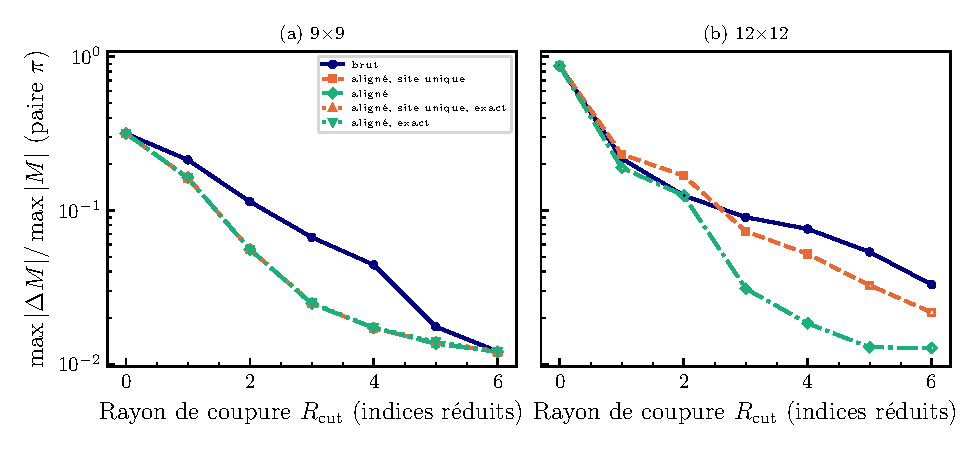
\includegraphics[width=\textwidth]{figures/fig_rcut_aligned.pdf}
    % À REVOIR : légende provisoire du 2026-10-05 ; étiquettes « site unique » / « Kumagai–Oba » de la figure à renommer (make_figures_controles.py)
    \caption[Erreur de troncature selon la référence du potentiel.]{Écart relatif maximal $\max|\Delta M|/\max|M|$ sur les blocs $\pi$--$\pi^*$ entre les éléments de matrice interpolés avec troncature à $R_\text{cut}$ et ceux obtenus avec toutes les cellules, pour (a) $9\times9$ et (b) $12\times12$, avec les matrices brutes, les matrices alignées de production (constante de Kumagai-Oba) et une variante alignée sur un seul site ; les courbes « exact » appliquent l'alignement au potentiel plutôt qu'aux blocs diagonaux de la base de Wannier et se superposent aux précédentes. C'est la quantité de la première ligne du tableau~\ref{tab:rcut_M}, pour tous les rayons de coupure.}
    \label{fig:rcut_aligned}
\end{figure}
\begin{figure}[htbp]
    \centering
    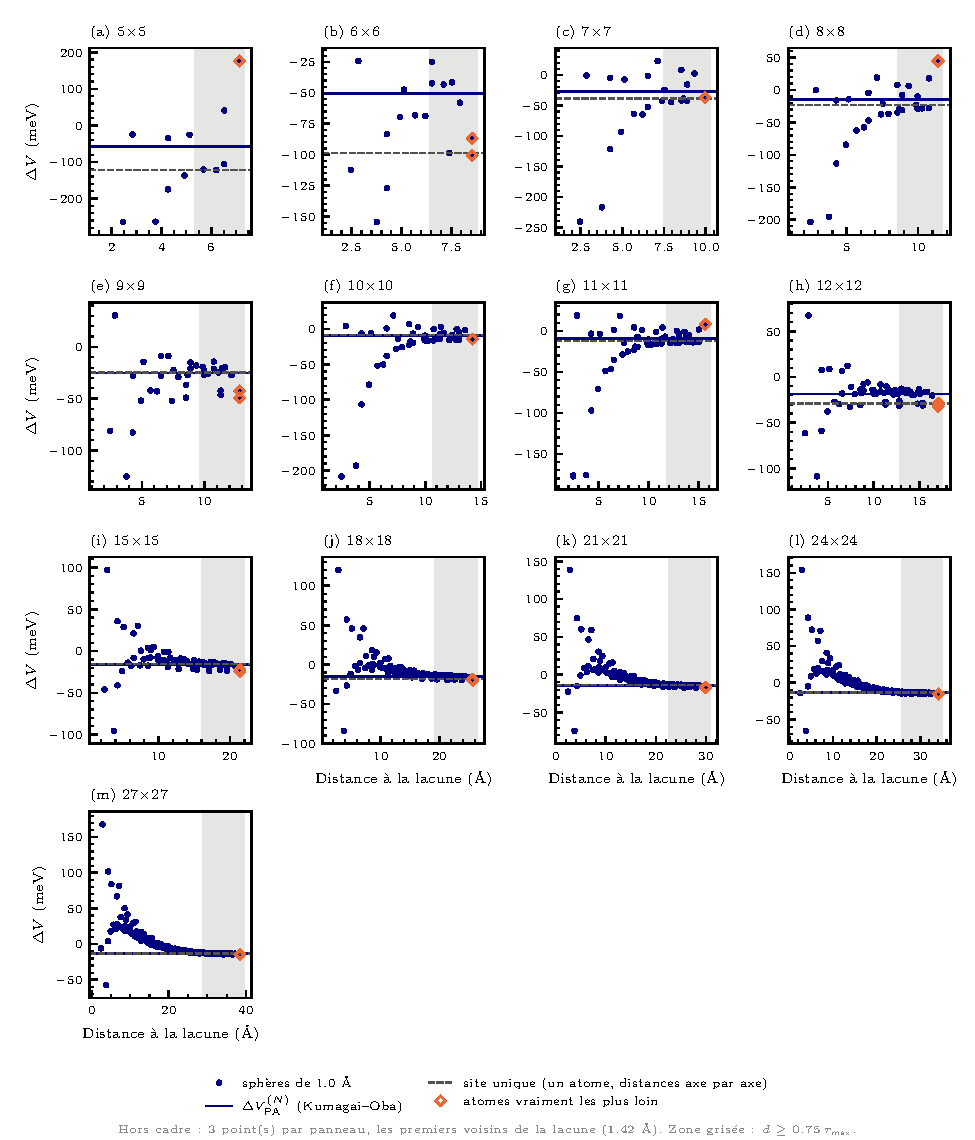
\includegraphics[width=\textwidth]{figures/fig_offset_profiles_13.pdf}
    % À REVOIR : légende provisoire du 2026-10-05 ; étiquettes « Kumagai–Oba » / « site unique » de la figure (make_figures_controles.py)
    \caption[Décalages de potentiel sur les sites atomiques pour treize tailles.]{Décalage du potentiel de la lacune $\Delta V_\alpha$ moyenné sur une sphère de $1.0$~\AA{} autour de chaque atome, en fonction de la distance à la lacune (image minimale), pour les treize tailles de super-cellule de $5\times5$ à $27\times27$. La zone grisée marque la région $d\ge0.75\,r_\text{max}$ dont la moyenne définit la constante d'alignement $\Delta V_\text{PA}^{(N)}$ (trait plein, prescription (A) du tableau~\ref{tab:alignement}) ; les tirets donnent la valeur du site unique le plus éloigné (prescription (D)) et les losanges marquent les atomes les plus éloignés.}
    \label{fig:offset_profiles_13}
\end{figure}
\begin{figure}[htbp]
    \centering
    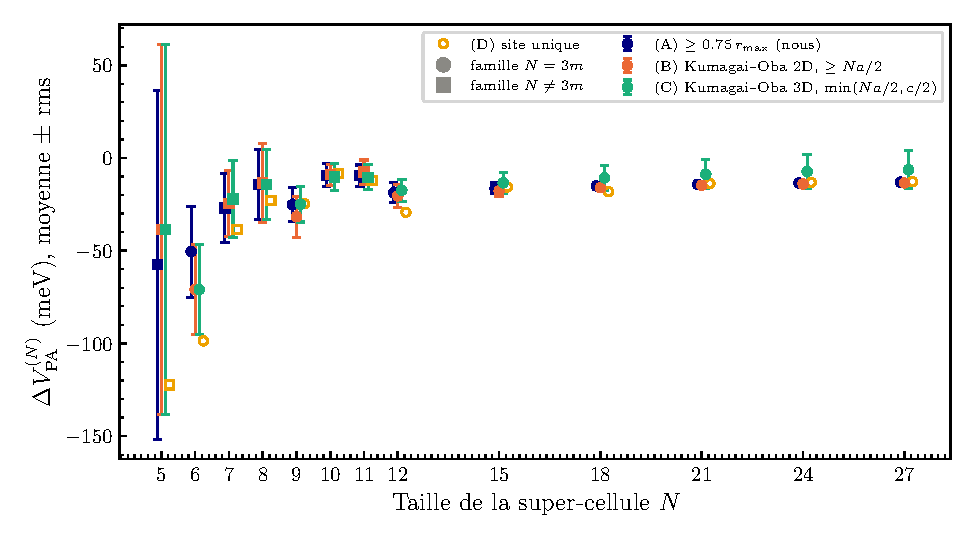
\includegraphics[width=\textwidth]{figures/fig_alignement_regions.pdf}
    % À REVOIR : légende provisoire du 2026-10-05
    \caption[Constante d'alignement selon la région d'échantillonnage.]{Constante d'alignement $\Delta V_\text{PA}^{(N)}$ (moyenne et écart-type des décalages de sphère) en fonction de la taille $N$ de la super-cellule, pour les quatre prescriptions du tableau~\ref{tab:alignement} : (A) $d\ge0.75\,r_\text{max}$ (production), (B) Kumagai-Oba à deux dimensions, $d\ge Na/2$, (C) Kumagai-Oba à trois dimensions, $d\ge\min(Na/2, c/2)$, et (D) site unique.}
    \label{fig:alignement_regions}
\end{figure}

\begin{figure}[htbp]
    \centering
    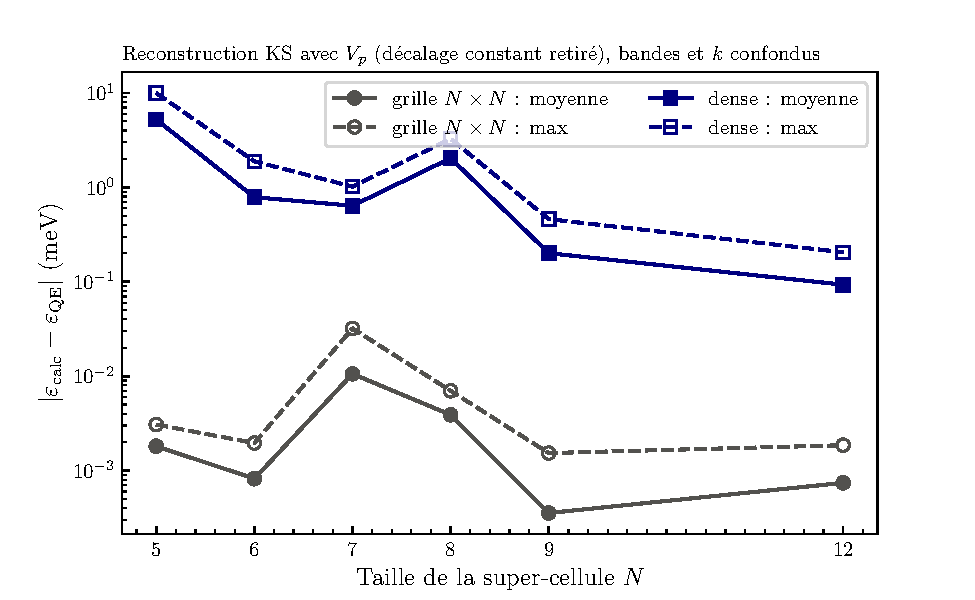
\includegraphics[width=\textwidth]{figures/fig_ks_reconstruction.pdf}
    \caption[Reconstruction des valeurs propres de Kohn-Sham.]{Écart
    entre les valeurs propres de Kohn-Sham reconstruites par la chaîne
    d'évaluation des éléments de matrice, appliquée au potentiel de la
    super-cellule parfaite, et celles de \texttt{QuantumESPRESSO}.
    La moyenne et le maximum sont sur toutes les bandes et tous les points $\kv$, après le retrait d'un décalage constant entre les deux références d'énergie. L'exercice est fait pour les grilles $N\times N$, où la densité convergée est la même pour les états et le potentiel, et pour les grilles élargies $pN\times pN$, où la densité autocohérente est différente.}
    \label{fig:ks_reconstruction}
\end{figure}
Pour les grilles grossières $N\times N$, où les états de Bloch et le potentiel proviennent du même calcul autocohérent, les valeurs propres de \texttt{QuantumESPRESSO} sont reproduites à 1.5--32 $\mu$eV près et les éléments hors diagonaux sont inférieurs à $10^{-6}$ en valeur relative. Ce test valide contre une référence indépendante du code le repliement des vecteurs $\Gv$, les facteurs de forme, les phases atomiques, la normalisation et les préfacteurs communs aux deux parties de la matrice de couplage. Seule la soustraction des deux super-cellules lui échappe. Sur les grilles élargies $pN\times pN$, l'écart atteint 0.21 à 10 meV, ce qui est attendu puisque les états de Bloch proviennent de la cellule unitaire avec la grille élargie $pN\times pN$ tandis que le potentiel vient du calcul de la super-cellule, dont l'échantillonnage à $\Gamma$ équivaut à une grille $N\times N$. Les densités autocohérentes ne sont donc pas identiques, et le potentiel n'est pas exactement celui dont les états de Bloch sont les états propres. Cette incohérence est inhérente à toute approche par super-cellule et ne pose pas de problème pour notre méthode.

Les autres tests sont des vérifications de cohérence interne. L'hermiticité des matrices de couplage est respectée à $10^{-14}$. Le remplissage par zéros préserve les coefficients de Fourier aux points coïncidents à $10^{-15}$. La transformée de Fourier $\kv\to\Rv\to\kv$ reproduit les éléments de matrice de départ à $10^{-14}$ près, et la transformée aller-retour Bloch$\to$Wannier$\to$Bloch (les équations~\eqref{eqn:M_wannier} et~\eqref{eqn:M_interp}) évaluée aux points de la grille grossière elle-même, à $10^{-15}$ près. Le seul écart supérieur au bruit numérique, de $10^{-3}$, apparaît en comparant les éléments de matrice des grilles grossières et élargies aux points $\kv$ communs. Cet écart a la même origine que l'écart de reconstruction sur les grilles élargies c'est-à-dire la différence entre les deux densités autocohérentes, et non la chaîne de calcul de $M$.
\begin{table}[htbp]
    \centering
    \small
    \setlength{\tabcolsep}{2pt}
    % À REVOIR : légende provisoire du 2026-10-03
    \caption[Vérifications de la chaîne de calcul de la matrice de
    couplage.]{Vérifications de la chaîne de calcul de la matrice $M$ : les tests et la quantité qu'ils contrôlent, la valeur obtenue et le seuil d'acceptation. Sauf mention contraire la valeur est celle de la super-cellule de référence $9\times9$ ; les reconstructions de Kohn-Sham, l'hermiticité et l'application directe de $V_\text{ed}$ sont données en fourchette ou en maximum sur les six tailles, et le test de convention intensive porte sur chaque famille de tailles.}
    \label{tab:tests_M}
    \begin{tabular}{l l l l}
    \hline\hline
    Test & Quantité & Valeur & Seuil \\
    \hline
    Reconstruction KS, grille $N\times N$             & $\max|\varepsilon_\text{calc}-\varepsilon_\text{QE}|$ & 1.5--32~$\mu$eV            & --- \\
    \quad éléments hors diagonaux                     & rel. à $\max|\varepsilon|$                            & $\le 1.3\times10^{-6}$     & --- \\
    Reconstruction KS, grille élargie                 & $\max|\varepsilon_\text{calc}-\varepsilon_\text{QE}|$ & 0.21--10~meV               & --- \\
    Hermiticité ($M$ élargi, six tailles)             & $\max|M-M^\dagger|/\max|M|$                           & $\le 2.3\times10^{-14}$    & $10^{-12}$ \\
    Application directe de $V_\text{ed}$, $N\times N$ & $\max|\Delta M|$, L et NL                             & $\le 3.3\times10^{-14}$~eV & $10^{-6}$~eV \\
    \quad grilles élargies                            & idem                                                  & $\le 1.2\times10^{-8}$~eV  & $10^{-6}$~eV \\
    Remplissage, coefficients coïncidents             & $\max|\Delta M^\text{L}|/\max|M^\text{L}|$            & $1.3\times10^{-15}$        & $10^{-10}$ \\
    Remplissage, points $\kv$ communs                 & écart rel. valeurs singulières                        & $1.3\times10^{-3}$         & $2\times10^{-3}$ \\
    Fourier $\kv\to\Rv\to\kv$                         & $\max|\Delta M|/\max|M|$                              & $2.4\times10^{-14}$        & $10^{-12}$ \\
    Bloch$\to$Wannier$\to$Bloch                       & écart rel. valeurs singulières                        & $1.3\times10^{-15}$        & $10^{-12}$ \\
    Convention intensive, $N = 6, 9, 12$              & $(\max-\min)/\text{moy.}$ de $\max|M|$                & $2.3\times10^{-2}$         & $5\times10^{-2}$ \\
    \quad $N = 5, 7, 8$                               & idem                                                  & $2.1\times10^{-2}$         & $5\times10^{-2}$ \\
    \hline\hline
\end{tabular}

\end{table}

\section{Convergence et vérifications de la matrice $T$}\label{sec:annexe_T_tests}

Cette section rassemble les preuves de convergence du schéma de l'amas de la matrice $T$ du chapitre~\ref{chap:T} : le rayon de coupure, la grille de sortie, l'élargissement et la grille interne de la fonction de Green de l'amas. Le corps du chapitre (section~\ref{sec:T_results}) ne garde que les paramètres retenus et les variations mesurées.

\begin{figure}[htbp]
    \centering
    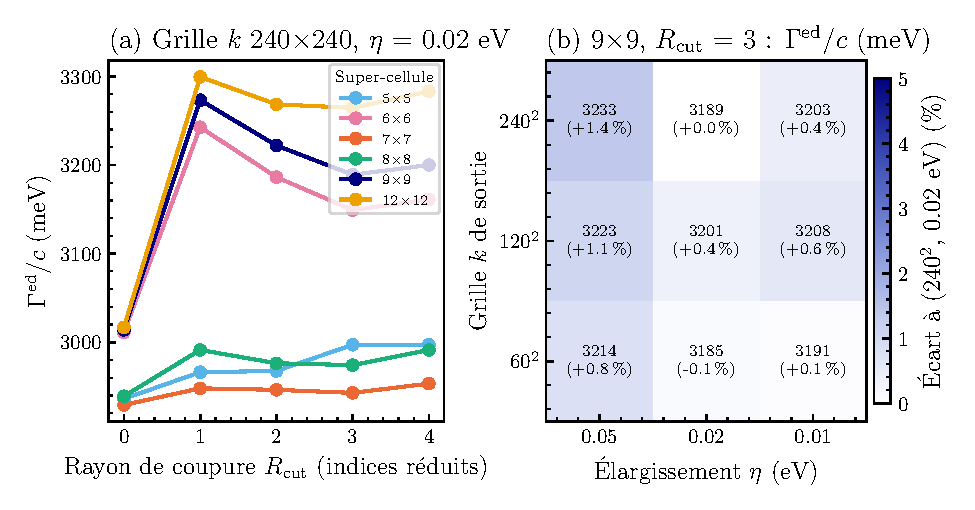
\includegraphics[width=\textwidth]{figures/fig_convergence.pdf}
    \caption[Convergence du taux d'amortissement par unité de
    concentration.]{Convergence de la médiane de $\Gamma^\text{ed}/c$
    sur $\pm3$~eV autour de $E_D$. (a) En fonction du rayon de coupure
    $R_\text{cut}$ du schéma de l'amas pour les six tailles de super-cellule,
    avec une grille de sortie $240\times240$ et un élargissement $\eta = 20$~meV. (b) En fonction de la grille de sortie et de $\eta$, pour la super-cellule de référence $9\times9$ à $R_\text{cut} = 3$. La couleur donne l'écart au point $(240^2, 20~\text{meV})$. La grille interne est de $300\times300$ ($N_{\tilde\kv}=300^2$) dans tous les cas.}
    \label{fig:convergence}
\end{figure}
\begin{table}[htbp]
    \centering
    \caption[Convergence du taux d'amortissement en fonction du rayon de
    coupure.]{Médiane de $\Gamma^\text{ed}/c$ (meV) sur $\pm3$~eV
    autour de $E_D$ en fonction du rayon de coupure $R_\text{cut}$, pour les
    six tailles de super-cellule (grille de sortie $240\times240$,
    $\eta = 20$~meV, grille interne $300\times300$). Nous distinguons les deux familles de super-cellules de la section~\ref{sec:M_détails}.}
    \label{tab:convergence_gamma}
    % Généré par scripts/make_tables.py : ne pas éditer (python scripts/make_tables.py --only convergence_gamma).
% tab:convergence_gamma, §4.3.5 → annexe D. Valeurs et sources cellule par cellule : tables/SOURCES.md.
% Sources : M2_plateau/level1_summary.csv
\begin{tabular}{c c ccccc}
    \hline\hline
    $N$ & $N \bmod 3$ & $R_\text{cut}=0$ & 1 & 2 & 3 & 4 \\
    \hline
    6  & 0 & 3011 & 3243 & 3186 & 3149 & 3161 \\
    9  & 0 & 3014 & 3273 & 3222 & 3189 & 3200 \\
    12 & 0 & 3017 & 3299 & 3269 & 3265 & 3283 \\
    \hline
    5  & 2 & 2936 & 2966 & 2968 & 2997 & 2997 \\
    7  & 1 & 2929 & 2948 & 2946 & 2943 & 2953 \\
    8  & 2 & 2939 & 2991 & 2976 & 2974 & 2991 \\
    \hline\hline
\end{tabular}

\end{table}
\begin{table}[htbp]
    \centering
    % À REVOIR : légende provisoire du 2026-10-04
    \caption[Convergence du taux d'amortissement en grille interne.]{Convergence en grille interne $N_{\tilde\kv}$ de la fonction de Green de l'amas~\eqref{eqn:g_loc}, pour la super-cellule de référence $9\times9$ et les paramètres de production ($R_\text{cut}=3$, grille de sortie $240^2$, $\eta=20$~meV) : médiane de $\Gamma^\text{ed}/c$ sur la fenêtre $\pm3$~eV et sur la zone $|\varepsilon-E_D|\le0.3$~eV, taux d'amortissement des états situés au point de Dirac et position $E_\text{res}$ de la résonance, définie comme l'énergie de l'état de la grille de sortie où $\Gamma^\text{ed}/c$ est maximal.}
    \label{tab:grille_interne}
    \begin{tabular}{c c c c c}
    \hline\hline
    & \multicolumn{2}{c}{Médiane de $\Gamma^\text{ed}/c$ (meV)} & $\Gamma^\text{ed}/c\,(E_D)$ & $E_\text{res}-E_D$ \\
    \cline{2-3}
    $N_{\tilde\kv}$ & $\pm3$~eV & $\pm0.3$~eV & (meV) & (eV) \\
    \hline
    $150^2$ & 3210 & 4289 & 5662 & $-0.238$ \\
    $300^2$ & 3189 & 3045 & 4287 & $-0.175$ \\
    $450^2$ & 3196 & 3080 & 4120 & $-0.175$ \\
    $600^2$ & 3192 & 3039 & 4090 & $-0.175$ \\
    \hline\hline
\end{tabular}

\end{table}
\begin{figure}[htbp]
    \centering
    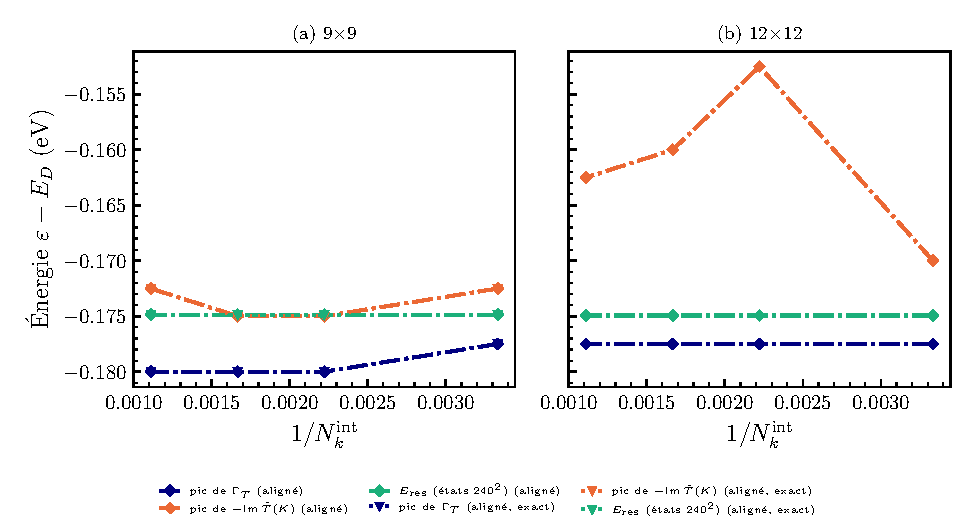
\includegraphics[width=\textwidth]{figures/fig_resonance_vs_nkint_plateau.pdf}
    % À REVOIR : légende provisoire du 2026-10-04 ; étiquettes « Kumagai–Oba » de la figure à renommer « aligné » (make_figures_controles.py)
    \caption[Position de la résonance en fonction de la grille interne.]{Position de la résonance de la lacune en fonction de l'inverse de la grille interne $N_k^\text{int}=N_{\tilde\kv}$, pour les super-cellules (a) $9\times9$ et (b) $12\times12$ et les matrices alignées, avec les paramètres de production : pic de la courbe $\Gamma_T(\varepsilon)$ obtenue par la moyenne lorentzienne~\eqref{eqn:moyenne_lorentzienne}, pic de $-\mathrm{Im}\,\bar T(K;\varepsilon)$ et $E_\text{res}$ (état de la grille de sortie $240^2$ où $\Gamma^\text{ed}/c$ est maximal). Pour $9\times9$, l'alignement appliqué aux blocs diagonaux de la base de Wannier (section~\ref{sec:M_détails}) et l'alignement exact du potentiel se superposent.}
    \label{fig:resonance_vs_nkint_plateau}
\end{figure}

\begin{table}[htbp]
    \centering
    \small
    \setlength{\tabcolsep}{4pt}
    % À REVOIR : légende provisoire du 2026-10-05
    \caption[Vérifications du schéma de l'amas.]{Vérifications de la chaîne
    de calcul de la matrice $T$ et du taux d'amortissement par le schéma de l'amas : les tests et la quantité qu'ils contrôlent, la valeur obtenue et le seuil d'acceptation. Le test de
    référence compare le schéma de l'amas à l'inversion dense de
    l'équation~\eqref{eqn:T_chap} dans le sous-espace des cinq fonctions
    de Wannier, pour la super-cellule $5\times5$. Le test de $\mathcal{G}^{(0)}_\mathcal{C}$ par lots compare la fonction de Green de l'amas~\eqref{eqn:g_loc} construite par lots d'énergies à son évaluation directe ; la positivité est vérifiée sur les états de la fenêtre $\pm3$~eV de la super-cellule de référence $9\times9$.}
    \label{tab:tests_T}
    % Généré par scripts/make_tables.py : ne pas éditer (python scripts/make_tables.py --only tests_T).
% tab:tests_T, §4.2.5 → annexe D. Valeurs et sources cellule par cellule : tables/SOURCES.md.
% Sources : M2_plateau/M_tests_summary.csv ; M2_plateau/nkint_check_9x9.csv ; M2_plateau/resonance_9x9.npz ; ch4/NOTES_TGAMMA.md
\begin{tabular}{l l l l}
    \hline\hline
    Test & Quantité & Valeur & Seuil \\
    \hline
    Référence, $5\times5$           & $\max|\Gamma_\text{loc}-\Gamma_\text{dense}|/\max\Gamma$ & $1.8\times10^{-13}$ & $10^{-8}$ \\
    Grille interne, $300^2\to600^2$ & écart rel. sur la médiane                                & $9.1\times10^{-4}$  & --- \\
    Positivité                      & $\min_{n\kv}\Gamma_{n\kv}N_\text{cells}$                 & $1.96$~eV           & $-10^{-8}$~eV \\
    \hline\hline
\end{tabular}

\end{table}
\begin{figure}[htbp]
    \centering
    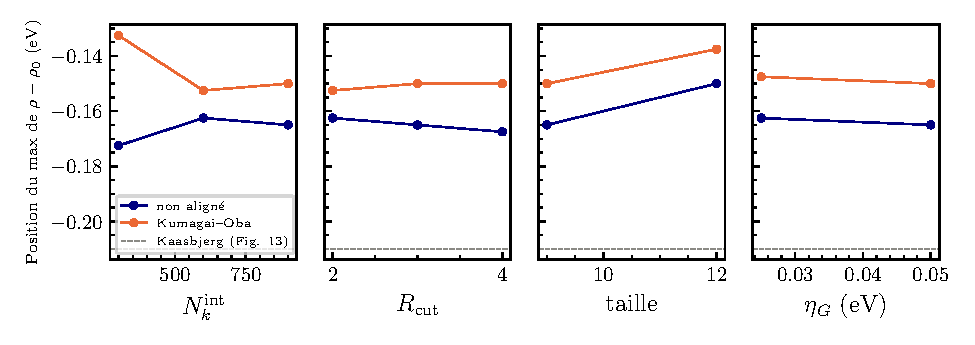
\includegraphics[width=\textwidth]{figures/fig_kaasbjerg_sensibilites.pdf}
    % À REVOIR : légende provisoire du 2026-10-05
    \caption[Sensibilité de la position du maximum de $\rho-\rho_0$.]{Position du maximum de $\rho-\rho_0$ de la densité d'états moyennée sur le désordre, à $c=1~\%$, en fonction de la grille interne, du rayon de coupure $R_\text{cut}$, de la taille de la super-cellule et de l'élargissement $\eta_G$, pour les matrices brutes et alignées. Les tirets marquent la valeur déduite de la figure 13 de Kaasbjerg~\cite{kaasbjergAtomisticMatrixTheory2020}, $-0.21$~eV.}
    \label{fig:kaasbjerg_sensibilites}
\end{figure}
\begin{figure}[htbp]
    \centering
    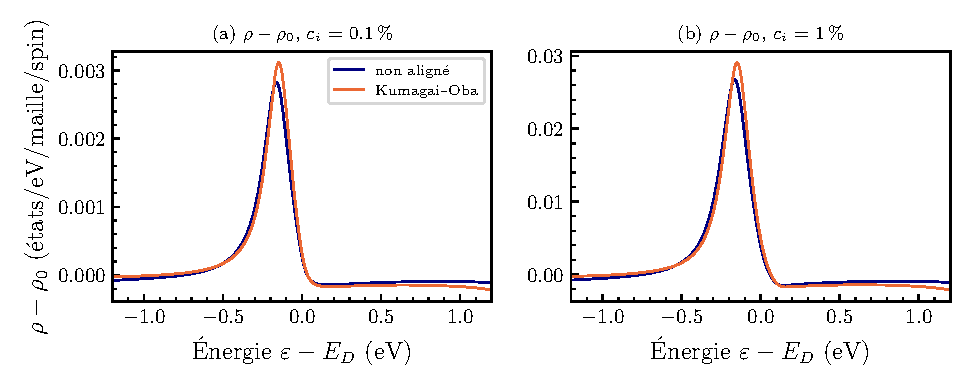
\includegraphics[width=\textwidth]{figures/fig_kaasbjerg_dos_c.pdf}
    % À REVOIR : légende provisoire du 2026-10-05 ; étiquettes « non aligné » / « Kumagai–Oba » de la figure à renommer « brut » / « aligné »
    \caption[Variation de la densité d'états moyennée sur le désordre.]{Variation $\rho-\rho_0$ de la densité d'états moyennée sur le désordre, grille $600^2$, $\eta_G=50$~meV, pour (a) $c=0.1~\%$ et (b) $c=1~\%$, matrices brutes et alignées de la super-cellule $9\times9$ ; c'est la quantité dont le tableau~\ref{tab:kaasbjerg} rapporte la position, la hauteur et la largeur du maximum.}
    \label{fig:kaasbjerg_dos_c}
\end{figure}

\section{Paramètres}

Cette section rassemble les paramètres numériques des six chaînes de calcul du mémoire, dans l'ordre des chapitres. Les calculs DFT et DFPT sont réalisés avec \texttt{QuantumESPRESSO} (version~7.4.1), l'interpolation par fonctions de Wannier avec \texttt{Wannier90} et \texttt{EPW}, et le post-traitement de la matrice de couplage électron-défaut en Python avec \texttt{NumPy} et \texttt{SciPy}.
% TODO P23 : versions d'EPW, de Wannier90, de NumPy et de SciPy absentes du texte des chapitres.
Tous les calculs ont été effectués sur la grappe Rorqual. Les fichiers d'entrée de chaque chaîne sont regroupés dans le dossier \texttt{calculs/} du dépôt GitHub \href{https://github.com/Gregb26/msc-graphene-raman-defects}{\texttt{msc-graphene-raman-defects}}, et le code de production dans \texttt{src/} du dépôt GitHub \href{https://github.com/Gregb26/graphene-raman}{\texttt{graphene-raman}}.
Dans chaque tableau, la colonne \og Section \fg{} renvoie à l'endroit du texte où la valeur est donnée. Une valeur qui diffère d'une chaîne à l'autre est donnée dans chaque tableau avec sa propre valeur.

\begin{table}[htbp]
    \centering
    \caption[Paramètres du calcul DFT de la cellule unitaire.]{Paramètres du calcul DFT de la cellule unitaire du graphène parfait (chapitre~\ref{chap:théorie}).}
    \label{tab:param_dft}
    \small
    \setlength{\tabcolsep}{4pt}
    \begin{tabular}{p{0.27\textwidth} p{0.46\textwidth} p{0.14\textwidth}}
        \hline\hline
        Paramètre & Valeur & Section \\
        \hline
        Code & \texttt{QuantumESPRESSO} & \ref{sec:electron_results} \\
        Fonctionnelle d'échange-corrélation & PBE & \ref{sec:electron_results} \\
        Pseudo-potentiel & ONCV \textit{stringent} pour le carbone, bibliothèque PseudoDojo & \ref{sec:electron_results} \\
        Coupure $E_\text{cut}$ & $100$~Ry & \ref{sec:electron_results} \\
        Grille $\kv$ & $27\times 27$, centrée sur $\Gamma$ & \ref{sec:electron_results} \\
        Occupation & Marzari-Vanderbilt, $\sigma = 0.01$~Ry & \ref{sec:electron_results} \\
        Diagonalisation & Davidson & \ref{sec:electron_results} \\
        \textit{Mixing} & Broyden, $\beta = 0.3$ & \ref{sec:electron_results} \\
        Seuil de convergence SCF & $10^{-14}$~Ry & \ref{sec:electron_results} \\
        Critère des tests de convergence & $0.1$~meV par atome & \ref{sec:electron_results} \\
        Paramètre de maille $a$ & $2.466$~\AA{}, par relaxation structurelle & \ref{sec:electron_results} \\
        Cellule de vide & & \\
        Troncature de Coulomb & & \\
        \hline\hline
    \end{tabular}
\end{table}

\begin{table}[htbp]
    \centering
    \caption[Paramètres des calculs DFPT et des phonons.]{Paramètres des calculs DFPT et des phonons du graphène parfait (chapitres~\ref{chap:théorie} et~\ref{chap:eph}).}
    \label{tab:param_dfpt}
    \small
    \setlength{\tabcolsep}{4pt}
    \begin{tabular}{p{0.27\textwidth} p{0.46\textwidth} p{0.14\textwidth}}
        \hline\hline
        Paramètre & Valeur & Section \\
        \hline
        Grille $\kv$ du calcul DFT préalable & $24\times 24$, centrée sur $\Gamma$ & \ref{sec:phonon_results} \\
        Grille $\qv$ de la DFPT & $24\times 24$ & \ref{sec:phonon_results} \\
        Occupation & Marzari-Vanderbilt, $\sigma = 0.02$~Ry & \ref{sec:phonon_results} \\
        Coupure $E_\text{cut}$ & $100$~Ry & \ref{sec:g_détails} \\
        Paramètre de maille & $2.466$~\AA & \ref{sec:g_détails} \\
        Cellule de vide & $30$~Bohr & \ref{sec:g_détails} \\
        Troncature de Coulomb & bidimensionnelle & \ref{sec:g_détails} \\
        Seuil de convergence (DFT et DFPT) & $10^{-14}$~Ry & \ref{sec:g_détails} \\
        Chemin d'interpolation & $\Gamma\to K\to M\to\Gamma$, $125$ points par segment & \ref{sec:phonon_results} \\
        Densité d'états : grille $\qv$ & $500\times 500$ & \ref{sec:phonon_results} \\
        Densité d'états : élargissement & gaussien, $3$~cm$^{-1}$ & \ref{sec:phonon_results} \\
        \hline\hline
    \end{tabular}
\end{table}

\begin{table}[htbp]
    \centering
    \caption[Paramètres des fonctions de Wannier.]{Paramètres des fonctions de Wannier de la cellule unitaire, pour la chaîne de la matrice $M$ (chapitre~\ref{chap:défauts}) et la chaîne de la matrice $g$ (chapitre~\ref{chap:eph}).}
    \label{tab:param_wannier}
    \small
    \setlength{\tabcolsep}{4pt}
    \begin{tabular}{p{0.27\textwidth} p{0.46\textwidth} p{0.14\textwidth}}
        \hline\hline
        Paramètre & Valeur & Section \\
        \hline
        Code (chaîne $M$) & \texttt{Wannier90} & \ref{sec:M_détails} \\
        Code (chaîne $g$) & \texttt{EPW}, qui fait appel à \texttt{Wannier90} & \ref{sec:g_détails} \\
        Grille (chaîne $M$) & grille élargie $pN\times pN$, soit $27\times 27$ pour la super-cellule de référence $9\times 9$ & \ref{sec:M_détails} \\
        Grille (chaîne $g$) & $24\times 24$ & \ref{sec:g_détails} \\
        Nombre de fonctions de Wannier & $5$ & \ref{sec:M_détails}, \ref{sec:g_détails} \\
        Fonctions d'essai & trois orbitales hybrides $sp^2$ et une orbitale $p_z$ sur un atome de carbone, une orbitale $p_z$ sur l'autre & \ref{sec:M_détails}, \ref{sec:g_détails} \\
        Fenêtre externe & $-25$~eV à $15$~eV & \ref{sec:M_détails}, \ref{sec:g_détails} \\
        Fenêtre gelée & jusqu'à $E_D + 2.5$~eV & \ref{sec:M_détails}, \ref{sec:g_détails} \\
        Étalements (chaîne $M$) & $0.61095$~\AA$^2$ ($\sigma$), $0.96695$~\AA$^2$ ($p_z$), total $3.76675$~\AA$^2$ & \ref{sec:M_détails} \\
        Étalements (chaîne $g$) & $0.6106$~\AA$^2$ ($\sigma$), $0.9655$~\AA$^2$ ($p_z$), total $3.7627$~\AA$^2$ & \ref{sec:g_détails} \\
        \hline\hline
    \end{tabular}
\end{table}

\begin{table}[htbp]
    \centering
    \caption[Paramètres des super-cellules et de la matrice $M$.]{Paramètres des calculs de super-cellules et de la matrice de couplage électron-défaut $M$ (chapitre~\ref{chap:défauts}).}
    \label{tab:param_M}
    \small
    \setlength{\tabcolsep}{4pt}
    \begin{tabular}{p{0.27\textwidth} p{0.46\textwidth} p{0.14\textwidth}}
        \hline\hline
        Paramètre & Valeur & Section \\
        \hline
        Tailles de super-cellule $N\times N$ & $N = 5, 6, 7, 8, 9, 12$ ; référence $9\times 9$ & \ref{sec:M_détails}, \ref{sec:M_results} \\
        Sous-réseau de la lacune & A pour $N = 5, 7, 8, 9$ ; B pour $N = 6, 12$ & \ref{sec:M_détails} \\
        Géométrie & non relaxée & \ref{sec:M_détails} \\
        Échantillonnage de la super-cellule & point $\Gamma$ seul & \ref{sec:M_détails} \\
        Grille grossière & $N\times N$ & \ref{sec:M_détails} \\
        Facteur d'élargissement $p$ & $5, 4, 4, 4, 3, 2$ pour $N = 5, 6, 7, 8, 9, 12$ & \ref{sec:M_détails} \\
        Grille élargie $pN\times pN$ & $pN = 25, 24, 28, 32, 27, 24$ & \ref{sec:M_détails} \\
        Fonctionnelle d'échange-corrélation & PBE & \ref{sec:M_détails} \\
        Pseudo-potentiel & ONCV \textit{stringent} pour le carbone, forme de Kleinman-Bylander, bibliothèque PseudoDojo & \ref{sec:M_détails} \\
        Coupure $E_\text{cut}$ & $100$~Ry & \ref{sec:M_détails} \\
        Occupation & Marzari-Vanderbilt, $\sigma = 0.01$~Ry & \ref{sec:M_détails} \\
        Seuil de convergence & $10^{-10}$~Ry sur l'énergie totale (super-cellules), $10^{-14}$~Ry (cellule unitaire) & \ref{sec:M_détails} \\
        Cellule de vide & $30$~Bohr & \ref{sec:M_détails} \\
        Troncature de Coulomb & bidimensionnelle & \ref{sec:M_détails} \\
        Rayon de coupure $R_\text{cut}$ & $3$, soit $29$ cellules unitaires & \ref{sec:M_results} \\
        Grille de sortie du test de troncature & $60\times 60$ & \ref{sec:M_results} \\
        Nombre de bandes & super-cellules : $2N^2$ bandes occupées et $30$ bandes vides ($N\le 18$) ou $5~\%$ de plus ($N\ge 21$), deux de moins avec la lacune ; cellule unitaire : $16$ (SCF) et $20$ (NSCF des grilles $\ge 24\times 24$) & \ref{sec:M_détails} \\
        Alignement du potentiel & Kumagai-Oba : moyenne des décalages de sphères de $1.0$~\AA{} sur les atomes à distance $d \ge 0.75\,r_\text{max}$ de la lacune (image minimale) ; soustrait des blocs diagonaux $M(\Rv,\Rv)$ des $N^2$ cellules dans la base de Wannier & \ref{sec:M_détails} \\
        Constante d'alignement $\Delta V_\text{PA}^{(N)}$ & $-57.6$, $-50.5$, $-26.9$, $-14.4$, $-25.1$, $-18.7$~meV pour $N = 5, 6, 7, 8, 9, 12$ ; incertitude $9.05$~meV pour $9\times 9$ & \ref{sec:M_results} \\
        \hline\hline
    \end{tabular}
\end{table}

\begin{table}[htbp]
    \centering
    \caption[Paramètres de la matrice $T$ et du taux d'amortissement $\Gamma^\text{ed}$.]{Paramètres du schéma de l'amas pour la matrice $T$ et le taux d'amortissement $\Gamma^\text{ed}$ (chapitre~\ref{chap:T}).}
    \label{tab:param_T}
    \small
    \setlength{\tabcolsep}{4pt}
    \begin{tabular}{p{0.27\textwidth} p{0.46\textwidth} p{0.14\textwidth}}
        \hline\hline
        Paramètre & Valeur & Section \\
        \hline
        Rayon de coupure $R_\text{cut}$ & $3$ & \ref{sec:T_détails} \\
        Nombre de cellules $N_L$ & $29$ (suite $1, 5, 13, 29, 49$ pour $R_\text{cut} = 0, \dots, 4$) & \ref{sec:T_détails} \\
        Nombre de fonctions de Wannier $N_W$ & $5$, soit une dimension $N_LN_W = 145$ & \ref{sec:T_détails} \\
        Grille interne $N_{\tilde\kv}$ & $300\times 300$ & \ref{sec:T_détails} \\
        Élargissement $\eta$ & $0.02$~eV & \ref{sec:T_détails} \\
        Grille de sortie $N_{\kv_f}$ & $240\times 240$, centrée sur $\Gamma$ & \ref{sec:T_détails} \\
        Fenêtre d'énergie & $\pm 3$~eV autour de $E_D$, soit $41\,266$ états & \ref{sec:T_détails} \\
        Pas de la grille d'énergie & $\eta/n_e$ avec $n_e = 8$, soit $2.5$~meV & \ref{sec:T_détails} \\
        Point de Dirac $E_D$ & $-4.239$~eV & \ref{sec:T_détails} \\
        Super-cellule de référence & $9\times 9$, grille élargie $27\times 27$ & \ref{sec:T_results} \\
        Moyenne lorentzienne & $\eta = 0.02$~eV & \ref{sec:T_results} \\
        Concentration de référence $c$ & $1~\%$ & \ref{sec:T_results} \\
        Comparaison avec Kaasbjerg & grille interne $900^2$ ; $\eta_G = 50$~meV ($\rho - \rho_0$, grille $600^2$) et $25$~meV ($A_\kv$) ; $\rho_0$ sur $1200^2$ avec $15$~meV ; $c = 0.1$ et $1~\%$ & \ref{sec:T_results} \\
        \hline\hline
    \end{tabular}
\end{table}

\begin{table}[htbp]
    \centering
    \caption[Paramètres de la chaîne \texttt{EPW}.]{Paramètres de la chaîne \texttt{EPW} pour la matrice $g$, le taux d'amortissement $\Gamma^\text{ep}$ et la largeur des phonons $\gamma_{\nu\qv}$ (chapitre~\ref{chap:eph}).}
    \label{tab:param_epw}
    \small
    \setlength{\tabcolsep}{4pt}
    \begin{tabular}{p{0.27\textwidth} p{0.46\textwidth} p{0.14\textwidth}}
        \hline\hline
        Paramètre & Valeur & Section \\
        \hline
        Grilles grossières $\kv$ et $\qv$ & $24\times 24$ et $24\times 24$ & \ref{sec:g_détails} \\
        Occupation (DFT et DFPT) & Marzari-Vanderbilt, $\sigma = 0.02$~Ry & \ref{sec:g_détails} \\
        Niveau de Fermi & $E_F = E_D = -4.2389$~eV & \ref{sec:g_détails} \\
        Fenêtre d'énergie & $\pm 3.5$~eV autour de $E_F$ & \ref{sec:g_détails} \\
        Grille de sortie pour $\Gamma^\text{ep}$ & $240^2$ points $\qv$, grille $\kv$ irréductible de même densité & \ref{sec:g_détails}, \ref{ssec:g_gamma_ep} \\
        Grille de sortie pour $\gamma_{\nu\qv}$ & $1200^2$ points $\kv$, $\qv$ le long de $\Gamma\to K\to M\to\Gamma$ & \ref{sec:g_détails}, \ref{ssec:g_gamma_ph} \\
        Élargissement gaussien $\sigma$ & $0.02$~eV & \ref{sec:g_détails} \\
        Températures & $300$~K et $10$~K & \ref{sec:g_détails} \\
        Moyenne lorentzienne de $\Gamma^\text{ep}(\varepsilon)$ & $\eta = 0.02$~eV & \ref{sec:g_détails} \\
        Convention de largeur & largeur totale $\gamma_{\nu\qv} = -2\,\mathrm{Im}\,\Pi_{\nu\qv}$, quantité imprimée par \texttt{EPW} & \ref{sec:g_détails}, \ref{ssec:g_gamma_ph} \\
        \hline\hline
    \end{tabular}
\end{table}
